\documentclass[11pt]{article}
\title{Meccano hexagons gallery}
\author{https://github.com/heptagons/meccano/hexa/gallery}
\date{2023/12/26}

\usepackage{../../meccano}
\usepackage{amssymb}
\usepackage{subcaption}

\begin{document}

\maketitle
\begin{abstract}
We build meccano\meccanoref rigid regular hexagons from sides $4$ to $24$. Hexagon perimeter has $6$ equal strips connected with $6$ bolts. To make it rigid we want to add a maximum of $3$ internal strips connected with at most $4$ extra bolts. The extra strips also must remain totally inside the perimeter, don't overlap with any other and must not be parallel to any external strip. With algebra and then sofware, we produce \texttt{hexagonal triangles} which have an internal angle of $120^\circ$ and we use their sides as the internal strips.
\end{abstract}

\section{Algebra and software}

\subsection{Hexagon triangles}

\begin{figure}[h]
\centering
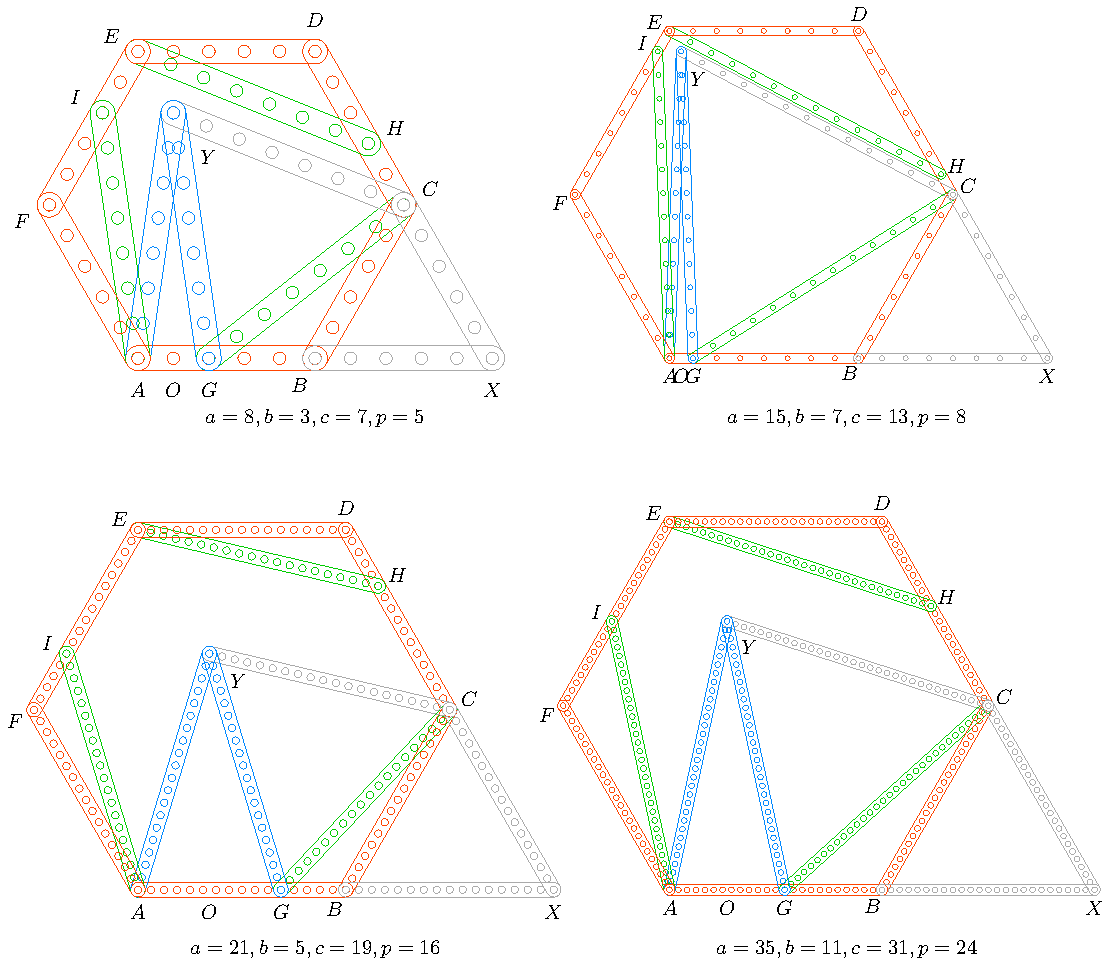
\includegraphics[scale=0.9]{build/hexa-builder-a}
\caption{First four cases where internal strip $c = \overline{GC}$ is an integer and makes rigid two consecutive regular hexagon sides $p = \overline{AB} = \overline{BC}$. Our software inspect two integers $a > b$ and looks for $c = \sqrt{a^2+b^2-ab}$ to be an integer. In the figures $b = \overline{GB}$ and $a = \overline{GX} = \overline{XJ} = \overline{JG} = p + b$. }
\label{fig:builder-a}
\end{figure}

We look for strips that can make rigid two consecutive internal sides the regular hexagon. Figure \ref{fig:builder-a} show the first four cases found. From any figure we have the internal hexagon angle is $\theta \equiv \angle{GBC} = 2\pi/3$. First we define the hexagon side as $p \equiv \overline{BC}$. From the triangle $\triangle{GBC}$ we define the other two sides as $b \equiv \overline{GB}$ and $c \equiv \overline{GC}$. Using the law of cosines and knowing that $\cos\theta = -1/2$ we have:
\begin{align}
c &= \sqrt{b^2 + p^2 - 2bp\cos\theta} \nonumber\\
 &= \sqrt{b^2 + p^2 - 2bp\left(-\frac{1}{2}\right)}
 = \sqrt{b^2 + p^2 + bp} \label{eq:triplet-cpb}
\end{align}

Then we defie $a \equiv p + b$ to get:
\begin{align}
c &= \sqrt{a^2 + b^2 - ab} \quad \texttt{ where } a > b
\end{align}

\begin{table}[H]
\begin{center}

% start go test ./hexa/. -run TestTriangles120Tex -v -count 1
\begin{tabular}{| c | c c c |}
\hline
$a$ & $c$ & $p$ & $b$ \\ [0.5ex]
\hline\hline
8 & 7 & 5 & 3 \\ \hline
15 & 13 & 8 & 7 \\ \hline
21 & 19 & 16 & 5 \\ \hline
35 & 31 & 24 & 11 \\ \hline
40 & 37 & 33 & 7 \\ \hline
48 & 43 & 35 & 13 \\ \hline
\end{tabular}
% end

\caption{\textbf{Hexagonal triangles} with sides $c > p > b$ with an internal angle $2\pi/3$.}
\label{tbl:triplets}
\end{center}
\end{table}

Our software iterates first $0 < a < max$ and then $1 < b < a$ and record all $c$ that is an integer. The first cases of such triangles with sides $c > p > b$ are shown table \ref{tbl:triplets} and we call them \textbf{Hexagonal triangles}.

Figure $\ref{fig:builder-a}$ shows hexagons of sizes $p = \{5,8,16,24\}$ with perimeter strips in orange made rigid adding three internal green strips of lenght $c = \{7,13,19,31\}$. 

\subsubsection{Hexagon height}

In figure $\ref{fig:builder-a}$ we have also an equilateral triangle $\triangle{GCY}$ and an isoscelles triangle $\triangle{AGY}$. The base of the isoscelles triangle is $x \equiv \overline{AG} = \overline{AB} - \overline{GB} = p - b$ and the equals sides are $\overline{AY} = \overline{GY} = c$. So we can calculate the height $y \equiv \overline{OY}$ substituting $c$ using equation \ref{eq:triplet-cpb}:
\begin{align}
y &= \sqrt{(\overline{GY})^2 - (\overline{AO})^2} \nonumber\\
 &= \sqrt{c^2 - \left(\frac{p - b}2\right)^2} \nonumber\\
 &= \sqrt{b^2 + p^2 + bp - \left(\frac{p-b}2\right)^2}
  = \frac{(p + b)\sqrt3}2 = \frac{a\sqrt3}2
\end{align}


% build-b
\begin{figure}[H]
\centering
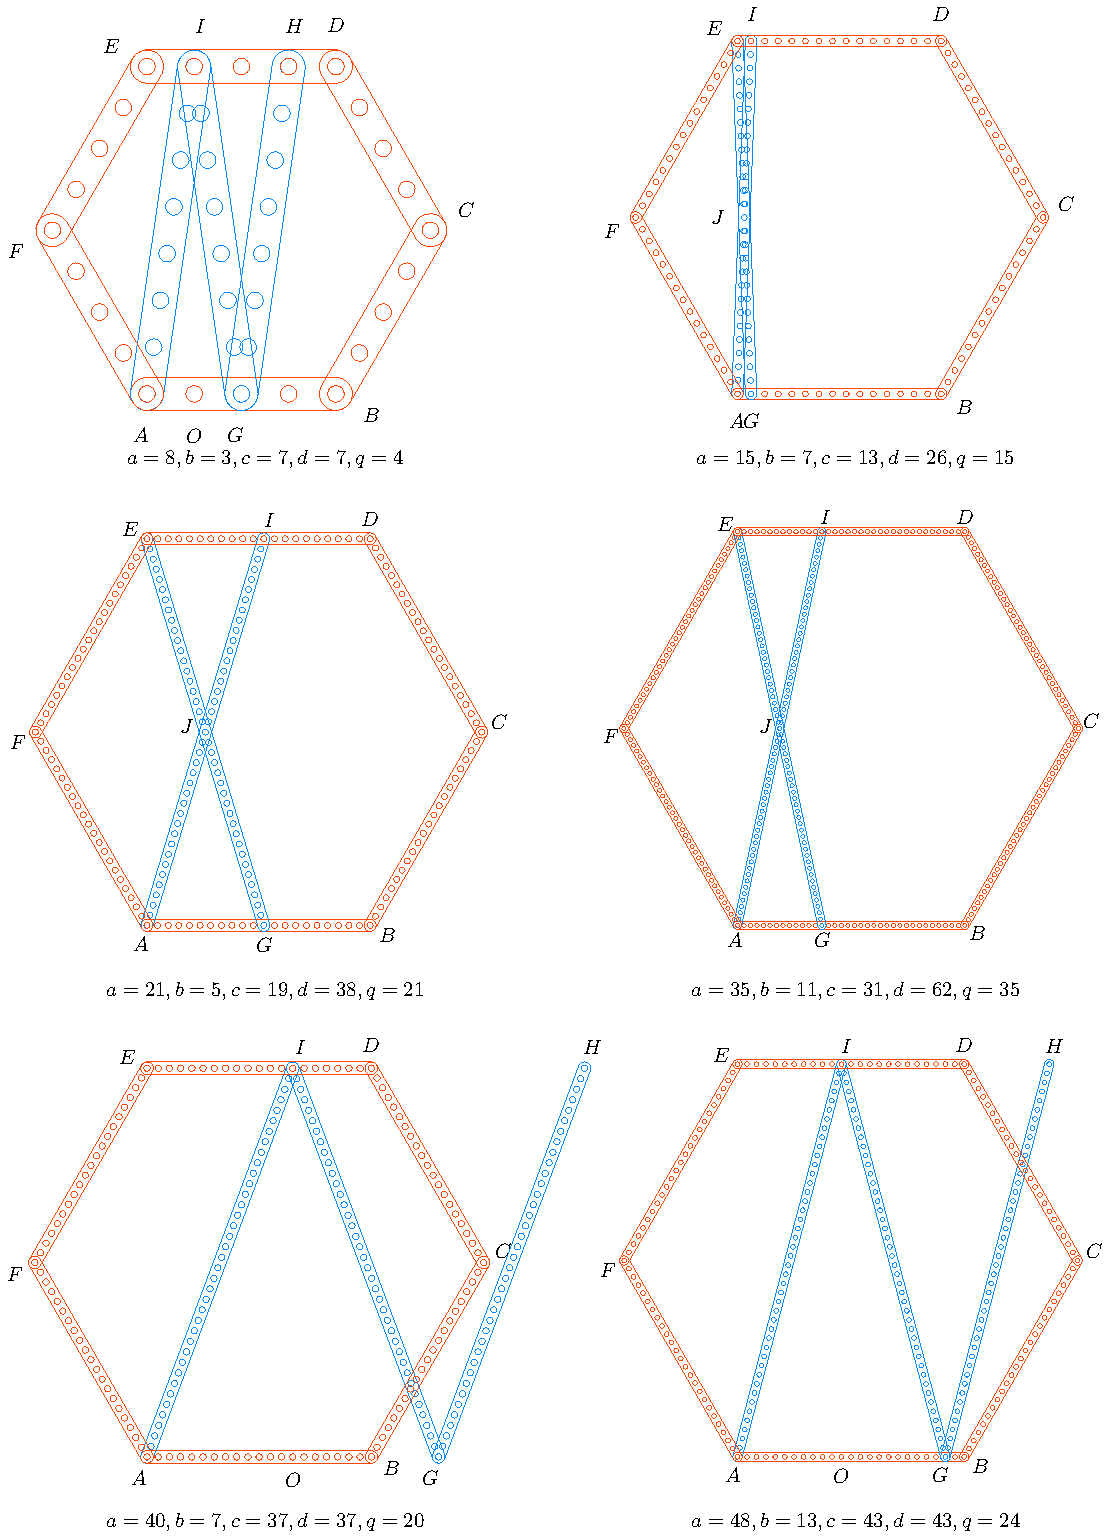
\includegraphics[scale=0.8]{build/hexa-builder-b}
\caption{First six cases of integral distances $c$. When the distance $p-b = \overline{AG}$ is even, we use the strips $d = c$ (in blue) to join opposites sides of hexagons of side $q = a/2$. When is odd, we use the strips $d = 2c$ (in purple) to join opposites sides of hexagons of side $q = a$.}
\label{fig:builder-b}
\end{figure}

We know $\dfrac{a\sqrt3}2$ is the height of the regular hexagon of side $\dfrac{a}2$ so we can use the blue strips to connect opposite sides. Figure \ref{fig:builder-b} show the smaller hexagons that have integer strips connecting opposites sides.

\subsubsection{Hexagon rigidity}

Through the gallery we will use the green, blue and purple strips and their copies multipled by integers as internal diagonals to make rigid regular hexagons from size $4$ to $24$. We prioritize minimum number of internal strips (2 or 3) and extra bolts (2 or 3 or 4) and the largest strips sizes as possible. We discard the hexagons which are scaled copies of smaller ones.

\section{Hexagons of size $s < 10$}

%4
\begin{figure}[H]
\centering
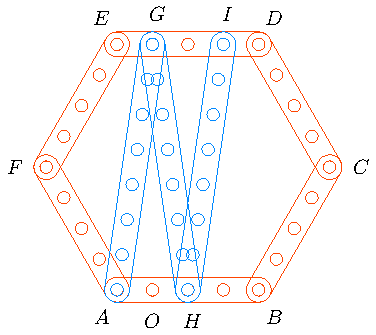
\includegraphics[scale=1]{4/hexa-4a}
\caption{Hexagon of size $4$ with three equal diagonals $\overline{GH} = \overline{HI} = \overline{IG} = 7$ and three extra bolts at vertices $G,H,I$.}
\label{fig:4a}
\end{figure}

Figure \ref{fig:4a} show a regular hexagon $ABCDEF$ of size $4$ with three diagonals of size $7$. We confirm the height of the hexagon with the distance $\overline{OG} = \sqrt{(\overline{AG})^2 - (\overline{AO})^2} = \sqrt{7^2 - 1^2} = 4\sqrt3$.

%5
\begin{figure}[H]
\centering
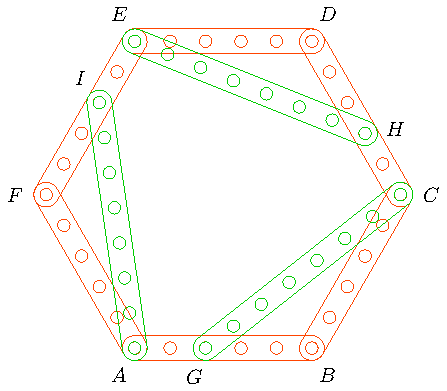
\includegraphics[scale=1]{5/hexa-5a}
\caption{Hexagon of size $5$ with three equal diagonals $\overline{GC} = \overline{HE} = \overline{IA} = 7$ and three extra bolts at vertices $G,H,I$.}
\label{fig:5a}
\end{figure}

Figure \ref{fig:5a} show a regular hexagon $ABCDEF$ of size $5$ with three diagonals of size $7$. We confirm the angle of $\alpha \equiv \angle{GBC} = 120^\circ$ with the law of cosines.
\begin{align}
\cos\alpha &= \frac{(\overline{GB})^2 + (\overline{BC})^2 - (\overline{GC})^2}
 {2(\overline{GB})(\overline{BC})}
 = \frac{3^2 + 5^2 - 7^2}{2(3)(5)} = -\frac{1}2 \nonumber
\end{align}

%8
\begin{figure}[H]
\centering
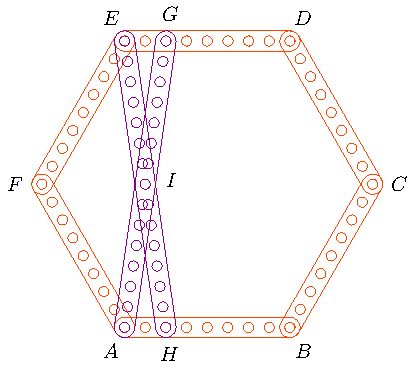
\includegraphics[scale=1]{8/hexa-8a}
\caption{Hexagon of size $8$ with \textbf{only} two diagonals $\overline{AH} = \overline{EI} = 14$ and three extra bolts at $G,H,I$.}
\label{fig:8a}
\end{figure}

Figure \ref{fig:8a} show hexagon $ABCDEF$ of size $8$. We confirm the height of the hexagon $\overline{AE} = \sqrt{(\overline{AG})^2 - (\overline{AH})^2} = \sqrt{14^2 - 2^2} = 8\sqrt3$.


%9
\begin{figure}[H]
\centering
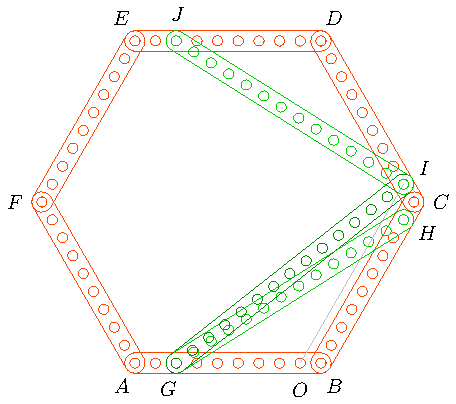
\includegraphics[scale=1]{9/hexa-9a}
\caption{Hexagon of size $9$ with three diagonals $\overline{GH} = \overline{IJ} = 13, \overline{GI} = 14$ and four extra bolts at $G,H,I,J$.}
\label{fig:9a}
\end{figure}

Figure \ref{fig:9a} show hexagon $ABCDEF$ of size $9$. Triangles $\triangle{HBG}$ and $\triangle{JID}$ have sides $(13,8,7)$ which are hexagonal triangles. Triangle $\triangle{GIO}$ has sides $(14,10,6)$ which is hexagonal triangle $(7,5,3)$ multipled by $2$.


%10
\begin{figure}[H]
\centering
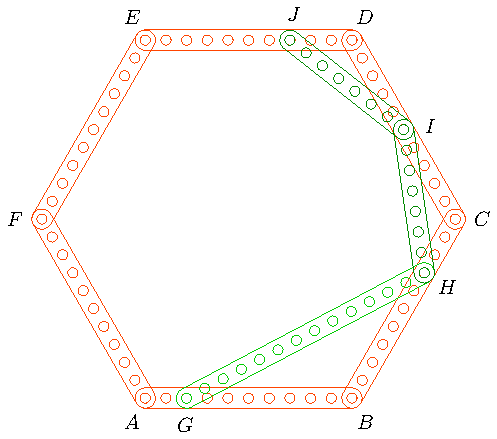
\includegraphics[scale=1]{10/hexa-10a}
\caption{Hexagon of size $10$ with three diagonals $\overline{HI} = \overline{IJ} = 7, \overline{GH} = 13$ and four extra bolts at vertices $G,H,I,J$.}
\label{fig:10a}
\end{figure}

Figure \ref{fig:10a} show hexagon $ABCDEF$ of size $10$. Triangles $\triangle{HIC}$ and $\triangle{JID}$ have sides $(7,5,3)$ which are hexagonal triangles. Triangle $\triangle{HGB}$ has size $(13,8,7)$ which is an hexagonal triangle.

\section{Hexagons of size $10 < s < 20$ }

% 11
\begin{figure}[H]
\centering
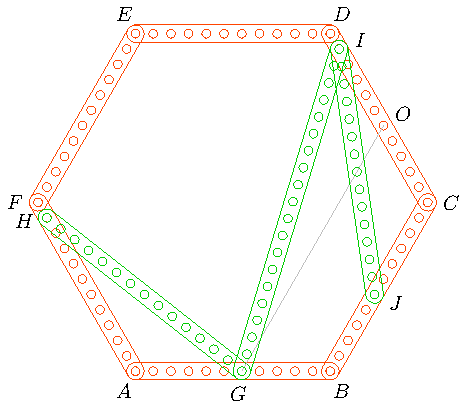
\includegraphics[scale=1]{11/hexa-11a}
\caption{Hexagon of size $11$ with three diagonals $\overline{GH} = \overline{IJ} = 14$ and $\overline{IG} = 19$ and four extra bolts at $G,H,I,J$.}
\label{fig:11a}
\end{figure}

Figure \ref{fig:11a} show hexagon $ABCDEF$ of size $11$. Triangles $\triangle{GHA}$ and $\triangle{JIC}$ have sides $(14,10,6)$ which are the hexagonal triangle $(7,5,3)$ multipled by 2. Triangle $\triangle{IGO}$ has sides $(19,16,5)$ which is an hexagonal triangle.

% 12
\begin{figure}[H]
\centering
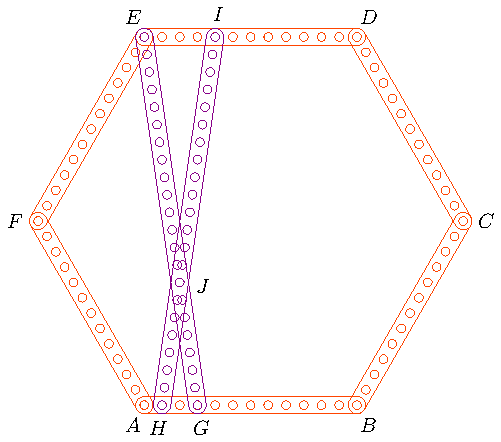
\includegraphics[scale=1]{12/hexa-12a}
\caption{Hexagon of size $12$ with \textbf{only} two diagonals $\overline{EG} = \overline{HI} = 21$ and four extra bolts at vertices $G,H,I,J$.}
\label{fig:12a}
\end{figure}

Figure \ref{fig:12a} show hexagon $ABCDEF$ of size $12$. We confirm the hexagon height: $\overline{AE} = \sqrt{(\overline{EG})^2 - (\overline{AG})^2} = \sqrt{21^2 - 3^2} = 12\sqrt3$.


% 13
\begin{figure}[H]
\centering
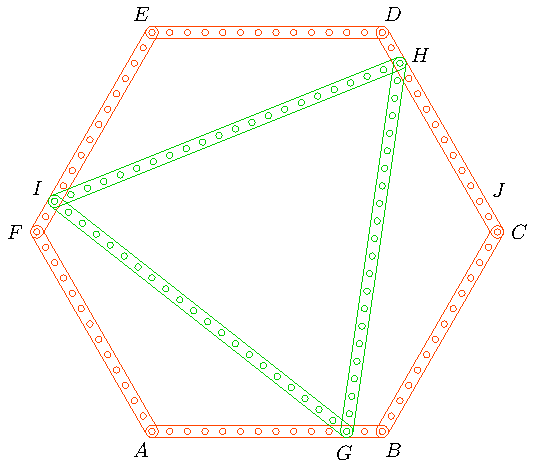
\includegraphics[scale=1]{13/hexa-13a}
\caption{Hexagon of size $13$ with three equal diagonals $\overline{GH} = \overline{HI} = \overline{IG} = 21$ forming an \textbf{equilateral triangle} and three bolts at vertices $G,H,I$.}
\label{fig:13a}
\end{figure}

Figure \ref{fig:13a} show hexagon $ABCDEF$ of size $13$. First we note the offset $o \equiv \overline{CO}$ which we use to calculate the sides $\{c,p,b\}$ of triangle $\triangle{GOH}$:
\begin{align}
o &\equiv \overline{DH} = \overline{CO} = 2 \nonumber\\
c &\equiv \overline{GH} = 21 \nonumber\\
p &\equiv \overline{GO} = \overline{BC} + o = 13+2 = 15 \nonumber\\
b &\equiv \overline{OH} = \overline{CD} - 2o = 13 - 2(2) = 9
\end{align}

The sides $c,p,b$ are $(21,15,9)$ which is hexagonal triangle $(7,5,3)$ multipled by $3$. For this case having an equilateral triangle inside the hexagon we can calculate $c$ in function of $s,o$ using the equation \ref{eq:triplet-cpb}:
\begin{align}
b &= s - 2o \nonumber\\
p &= s + o \nonumber\\
c &= \sqrt{b^2 + p^2 - bp} \nonumber\\
   &= \sqrt{(s - 2o)^2 + (s+o)^2 + (s - 2o)(s+o)} \nonumber\\
   &= \sqrt{3s^2 - 3so + 3o^2}
\end{align}

Using the formula our software found more cases shown in the table \ref{tbl:eqtriangles}
\begin{table}[H]
\begin{center}
\begin{tabular}{| c c | c c c |} 
 \hline
 $s$ & $o$ & $c$ & $p$ & $b$ \\ [0.5ex] 
 \hline\hline
  13 &  2 &  21 &  15 &  9 \\ \hline
  23 &  1 &  39 &  24 & 21 \\ \hline
  37 & 11 &  57 &  48 & 15 \\ \hline
  59 & 13 &  93 &  72 & 33 \\ \hline
\end{tabular}
\caption{Hexagons of size $s$ with inside equilateral triangles of side $c$.}
\label{tbl:eqtriangles}
\end{center}
\end{table}

% 14
\begin{figure}[H]
\centering
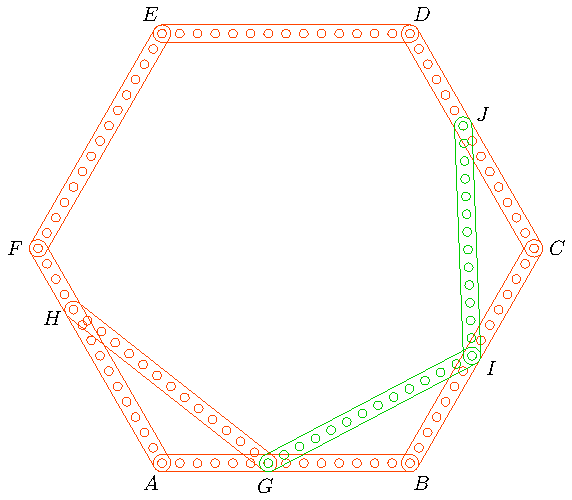
\includegraphics[scale=1]{14/hexa-14a}
\caption{Hexagon of size $14$ with three diagonals $\overline{GH} = 14, \overline{GI} = \overline{IJ} = 13$ and four extra bolts at vertices $G,H,I,J$.}
\label{fig:14a}
\end{figure}

Figure \ref{fig:14a} show hexagon $ABCDEF$ of size $14$. Triangle $\triangle{GHA}$ has sides $(14,10,6)$ which is hexagonal triangle $(7,5,3)$ multipled by $2$. Triangles $\triangle{IGB}$ and $\triangle{JCI}$ have sides $(13,8,7)$ which are hexagonal triangles.


% 15
\begin{figure}[H]
\centering
\begin{subfigure}{0.49\textwidth}
 \centering
 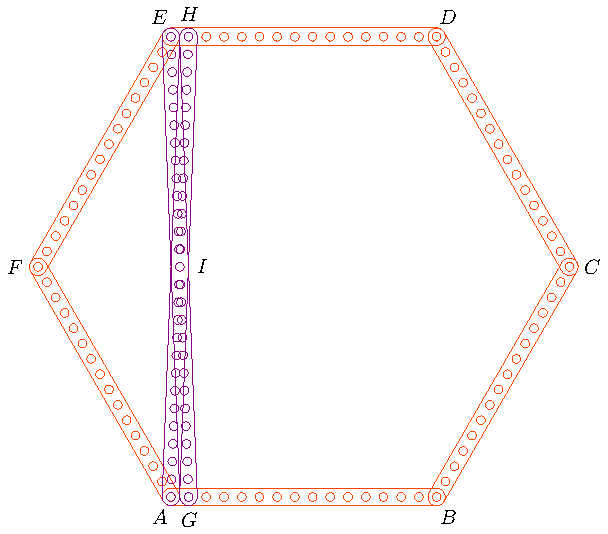
\includegraphics[scale=0.8]{15/hexa-15a}
 \caption{With \textbf{only} two diagonals. }
\end{subfigure}
\begin{subfigure}{0.49\textwidth}
 \centering
 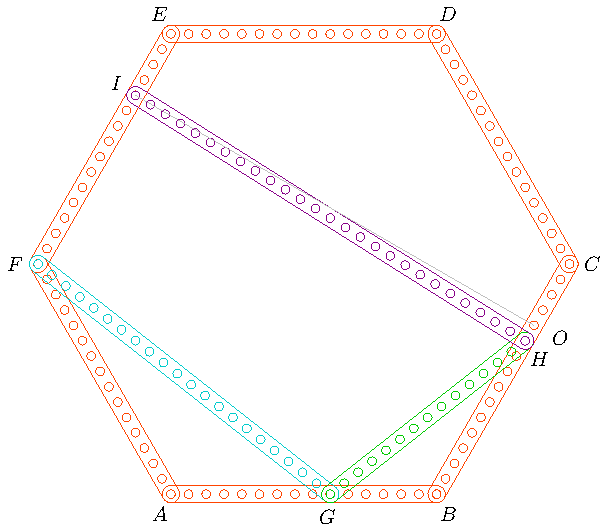
\includegraphics[scale=0.8]{15/hexa-15b}
 \caption{With three diagonals. }
\end{subfigure}
\caption{Hexagons of size $15$. (a) with diagonals $\overline{AH} = \overline{EG} = 26$ and three extra bolts at vertices $G,H,I$. (b) with diagonals $\overline{GF} = 21, \overline{GH} = 19, \overline{HI} = 26$ and three extra bolts at vertices $G,H,I$.}
\label{fig:15ab}
\end{figure}

Figure \ref{fig:15ab} show two hexagons $ABCDEF$ of size $15$. Hexagon height at (a) is $\overline{AE} = \sqrt{(EG)^2 - (AG)^2} = \sqrt{26^2 - 1^2} = 15\sqrt3.$ For hexagon at (b) we have that triangle $\triangle{GFA}$ sides are $(21,15,9)$ which are hexagonal triangle $(7,5,3)$ multipled by $3$; triangle $\triangle{GHB}$ sides are $(14,10,6)$ which is hexagonal triangle $(7,5,3)$ multipled by $2$; triangle $\triangle{HIO}$ is rectangle where $\overline{IO} = \sqrt{(\overline{HI})^2 - (\overline{HO})^2} = \sqrt{26^2 - 1^2} = 15\sqrt3$.

% 16
\begin{figure}[H]
\centering
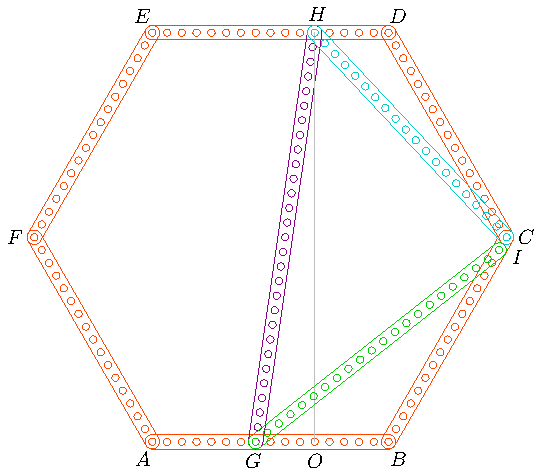
\includegraphics[scale=1]{16/hexa-16a}
\caption{Hexagon of size $16$ with three diagonals $\overline{GH} = 28, \overline{GI} = 21, \overline{CH} = 19$ and three extra bolts at $G,H,I$.}
\label{fig:16a}
\end{figure}

Figure \ref{fig:16a} show hexagon $ABCDEF$ of size $16$. Hexagon's height is $\overline{OH}=\sqrt{(\overline{GH})^2-(\overline{GO})^2}=\sqrt{28^2-4^2}=16\sqrt3$. Triangle $\triangle{IBG}$ sides are $(21,15,9)$ which is hexagonal triangle $(7,5,3)$ multipled by $3$. Triangle $\triangle{HCD}$ sides are $(19,16,5)$ which is an hexagonal triangle.


% 17
\begin{figure}[H]
\centering
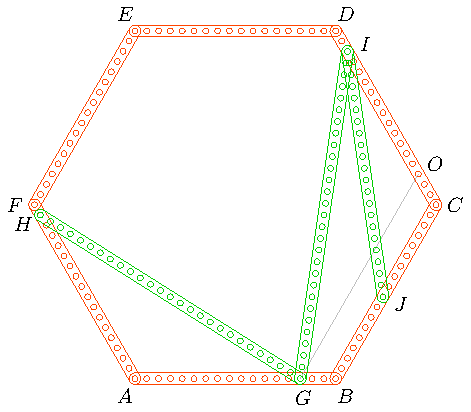
\includegraphics[scale=1]{17/hexa-17a}
\caption{Hexagon of size $17$ with three diagonals $\overline{GH} = 26, \overline{GI} = 28, \overline{IJ} = 21$ and four bolts at vertices $G,H,I,J$.}
\label{fig:17a}
\end{figure}

Figure \ref{fig:17a} show hexagon $ABCDEF$ of size $17$. Triangle $\triangle{GHA}$ sides are $(26,16,14)$ which is hexagonal triangle $(13,8,7)$ multiplied by $2$. Triangle $\triangle{IGO}$ sides are $(28,20,12)$ which is hexagonal triangle $(7,5,3)$ multipled by $4$. Triangle $\triangle{JIC}$ has sides $(21,15,9)$ which is hexagonal triangle $(7,5,3)$ multiplied by $3$.

% 18
\begin{figure}[H]
\centering
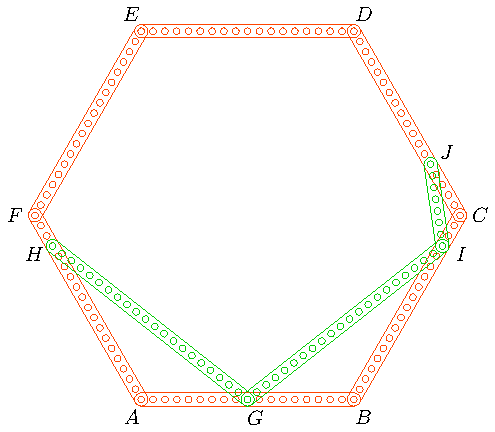
\includegraphics[scale=1]{18/hexa-18a}
\caption{Hexagon of size $18$ with three diagonals $\overline{GH} = \overline{GI} = 21, \overline{IJ} = 7$ and four extra bolts at vertices $G,H,I,J$.}
\label{fig:18a}
\end{figure}

Figure \ref{fig:18a} show hexagon $ABCDEF$ of size $18$. Triangles $\triangle{GHA}$ and $\triangle{GIB}$ have sides $(21,15,9)$ which are hexagonal triangles $(7,5,3)$ multipled by $3$. Triangle $\triangle{IJC}$ sides are $(7,5,3)$ which is an hexagonal triangle.


% 19
\begin{figure}[H]
\centering
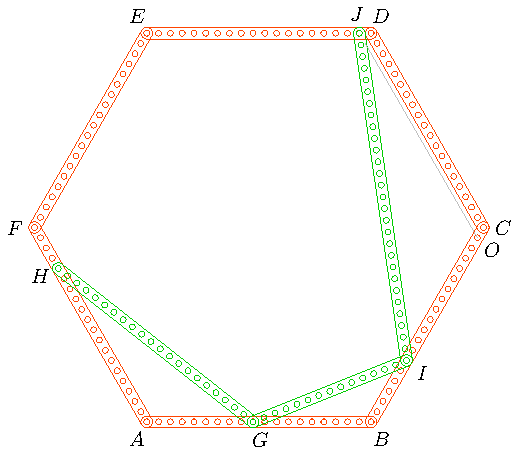
\includegraphics[scale=1]{19/hexa-19a}
\caption{Hexagon of size $19$ with three diagonals $\overline{GH} = 21, \overline{GI} = 14, \overline{IJ} = 28$ and four bolts at vertices $G,H,I,J$.}
\label{fig:19a}
\end{figure}

Figure \ref{fig:19a} show hexagon $ABCDEF$ of size $19$. Triangle $\triangle{GHA}$ has sides $(21,15,9)$ which correspond to hexagonal triangle $(7,5,3)$ multipled by $3$. Triangle $\triangle{GIB}$ has sides $(14,10,6)$ which correspond to hexagonal triangle $(7,5,3)$ multipled by $2$. Triangle $\triangle{IJO}$ has sides $(28,20,12)$ which correspond to hexagonal triangle $(7,5,3)$ multipled by $4$.

\section{Hexagons of size $\ge 20$}

% 20
\begin{figure}[H]
\centering
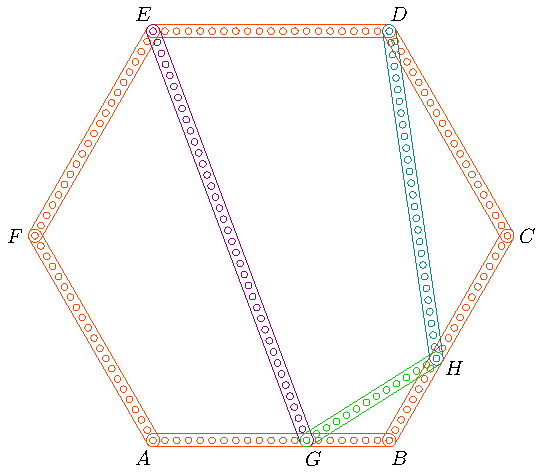
\includegraphics[scale=1]{20/hexa-20a}
\caption{Hexagon of size $20$ with three diagonals $\overline{GH} = 13$, $\overline{HD} = 28$ and $\overline{EG} = 37$ and \textbf{only} two extra bolts at vertices $G$ and $H$.}
\label{fig:20a}
\end{figure}

Figure \ref{fig:20a} show regular hexagon $ABCDEF$ of size $20$. Triangle $\triangle{GBH}$ sides are $(13,8,7)$ which is an hexagonal triangle. Triangle $\triangle{HCD}$ sides are $(28,20,12)$ which is hexagonal triangle $(7,5,3)$ multiplied by $4$. Right triangle $\triangle{EAG}$ side $\overline{AE} = \sqrt{(\overline{EG})^2 - (\overline{AG})^2} = \sqrt{37^2 - 13^2} = 20\sqrt3$ equals to hexagon height.

% 21
\begin{figure}[H]
\centering
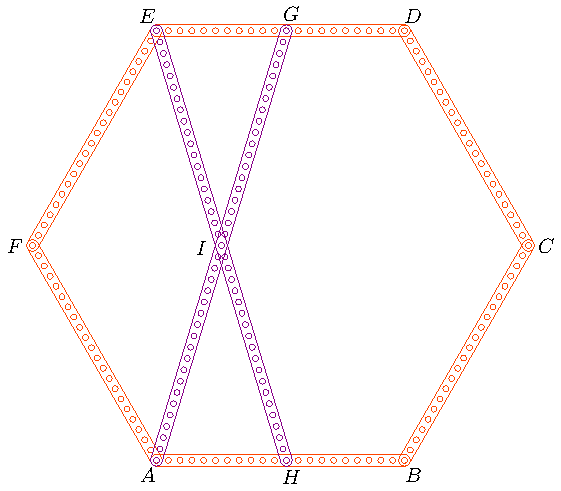
\includegraphics[scale=1]{21/hexa-21a}
\caption{Hexagon of size $21$ with \textbf{only} two diagonals $\overline{AG} = \overline{EH} = 38$. Segments $\overline{AH} = \overline{EG} = 11$, segment $\overline{AI} = 19$. Three extra bolts at $H,G,I$.}
\label{fig:21a}
\end{figure}

Figure \ref{fig:21a} show regular hexagon $ABCDEF$ of size $21$. We confirm the height of the hexagon is $\overline{AE} = \sqrt{(\overline{EH})^2 - (\overline{AH})^2} = \sqrt{38^2 - 11^2} = 21\sqrt3$.

% 22
\begin{figure}[H]
\centering
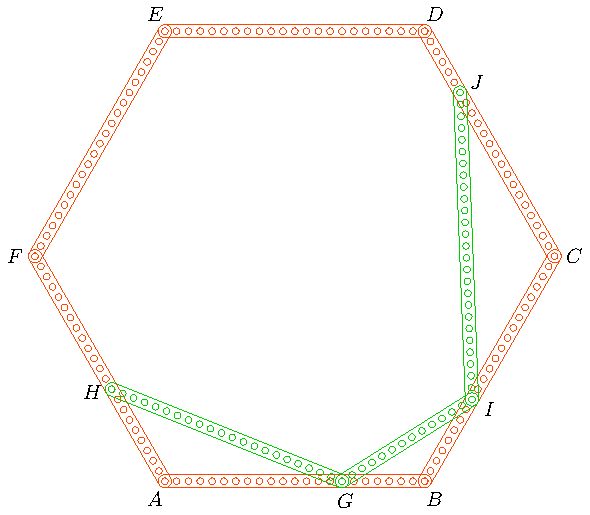
\includegraphics[scale=0.9]{22/hexa-22a}
\caption{Hexagon of size $22$ with three diagonals $\overline{GH} = 21, \overline{GI} = 13, \overline{IJ} = 26$ and four extra bolts at vertices $H,G,I,J$.}
\label{fig:22a}
\end{figure}

Figure \ref{fig:22a} show regular hexagon $ABCDEF$ of size $22$. Triangle $\triangle{GHA}$ sides are $(21,15,9)$ which is hexagonal triangle $(7,5,3)$ multiplied by $3$. Triangle $\triangle{GIB}$ sides are $(13,8,7)$ which is an hexagonal triangle. Triangle $\triangle{IJC}$ sides are $(26,16,14)$ which is hexagonal triangle $(13,8,7)$ multiplied by $2$.

% 23
\begin{figure}[H]
\centering
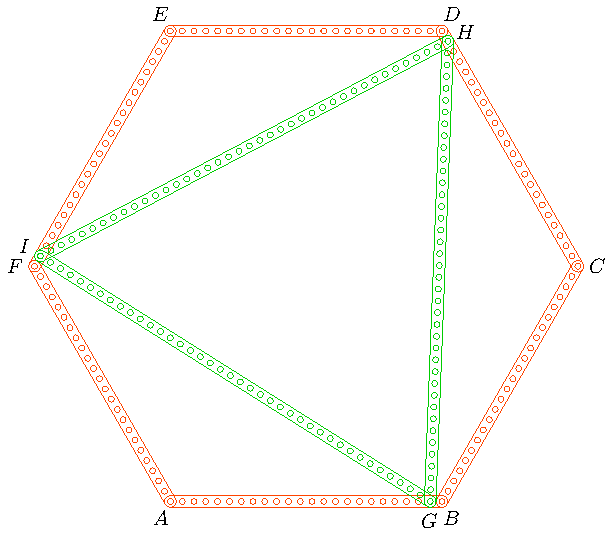
\includegraphics[scale=0.9]{23/hexa-23a}
\caption{Hexagon of size $23$ with three equal diagonals $\overline{GH} = \overline{HI} = \overline{IG} = 39$ forming and \textbf{equilateral triangle} with three extra bolts at vertices $G,H,I$.}
\label{fig:23a}
\end{figure}

Figure \ref{fig:23a} show a regular hexagon $ABCDEF$ of size $s=23$. Is the second hexagon having an equilateral triangle inside, in this case of size $c=39$ and described in table \ref{tbl:eqtriangles}.

% 24
\begin{figure}[H]
\centering
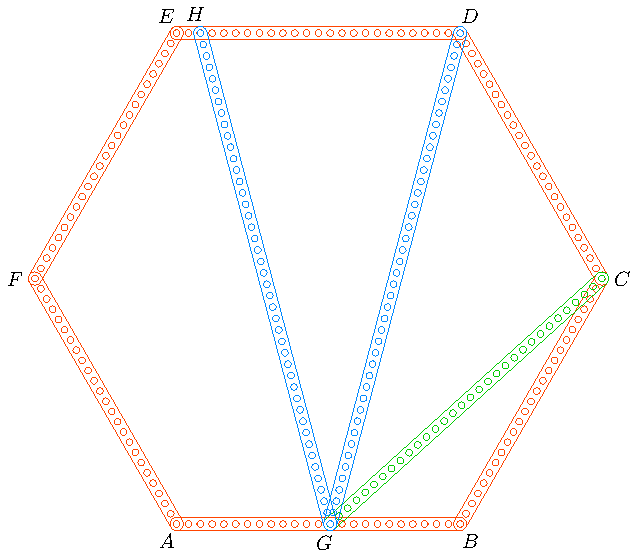
\includegraphics[scale=0.9]{24/hexa-24a}
\caption{Hexagon of size $24$ with diagonals $\overline{GC} = 31$ and $\overline{GD} = \overline{GH} = 43$ with \textbf{only} two extra bolts at vertices $G$ and $H$. Segments $\overline{GB} = 11$ and $\overline{DH} = 22$.}
\label{fig:24a}
\end{figure}

Figure \ref{fig:24a} show regular hexagon $ABCDEF$ of size $24$. Triangle $\triangle{GBC}$ has sides $\{31,24,11\}$ which is an hexagonal triangle in table \ref{tbl:triplets}. Triangle $\triangle{DHG}$ is the isoscelles triangle shown in figure \ref{fig:builder-b} case $a=48$ where $\overline{BD} = \sqrt{(\overline{DG})^2 - (\overline{GB})^2} = \sqrt{43^2 - 11^2} = 24\sqrt3$.



\end{document}
